\chapter{Implementation}

In this chapter we describe how the design of Chapter~\ref{ch:project} is realized in
code: the platform and language, the resulting project structure, the choices made while
implementing the protocol that were not fixed by the requirements, and the implementation
details of the protocol that were deliberately left out of the previous chapter.

\section{Platform}

The system is implemented in Gleam\footnote{https://gleam.run} 1.17, a statically typed
functional language that compiles to the Erlang Virtual Machine (BEAM) and interoperates
with OTP (\texttt{gleam\_otp} 1.2, \texttt{gleam\_erlang} 1.3). This choice follows
directly from the algorithm's own model: one asynchronous process per network node,
communicating only through message passing, with no shared state. This is precisely the
actor model natively provided by the BEAM.

\section{Project structure}

\begin{figure}[htbp]
\centering
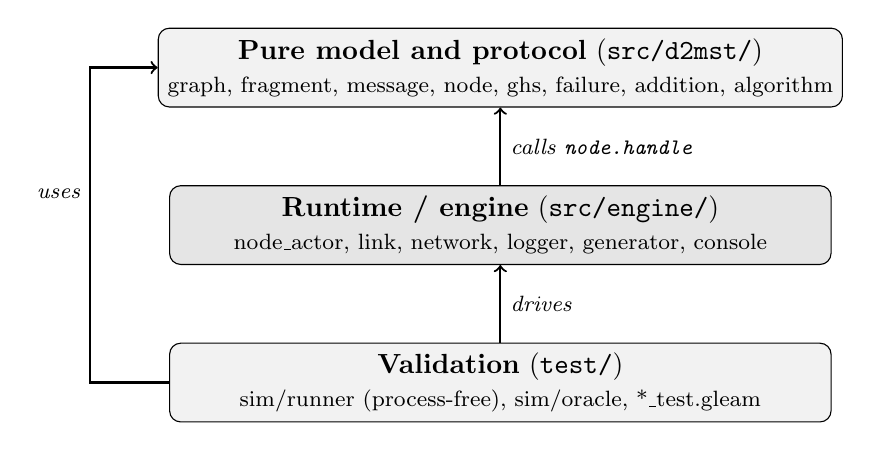
\begin{tikzpicture}[
    box/.style={draw, rounded corners, minimum width=8.4cm, minimum height=1cm, align=center},
    lbl/.style={font=\footnotesize\itshape}
]
\node[box, fill=black!5] (protocol) at (0,4) {\textbf{Pure model and protocol} (\texttt{src/d2mst/})\\
\footnotesize graph, fragment, message, node, ghs, failure, addition, algorithm};
\node[box, fill=black!10] (engine) at (0,2) {\textbf{Runtime / engine} (\texttt{src/engine/})\\
\footnotesize node\_actor, link, network, logger, generator, console};
\node[box, fill=black!5] (test) at (0,0) {\textbf{Validation} (\texttt{test/})\\
\footnotesize sim/runner (process-free), sim/oracle, *\_test.gleam};

\draw[->, thick] (test) -- node[right, lbl] {drives} (engine);
\draw[->, thick] (test.west) -- ++(-1,0) |- node[pos=0.3, left, lbl, align=right] {uses} (protocol.west);
\draw[->, thick] (engine) -- node[right, lbl] {calls \texttt{node.handle}} (protocol);
\end{tikzpicture}
\caption{The three-layer split. Protocol code has no notion of processes; the engine is
the only layer that touches them; validation exercises both, either directly or through
the process-free simulator.}
\label{fig:layers}
\end{figure}

The codebase follows the three-layer split of Figure~\ref{fig:layers}. This separation is
chosen so that the protocol, the part of the system whose correctness matters most, can be
understood, tested, and reasoned about independently of processes, scheduling, or message
loss.

\subsection{Pure model and protocol (\texttt{src/d2mst/})}

Every module in this layer is a pure function of its inputs; none of them import
\texttt{gleam/erlang/process} or \texttt{gleam/otp/actor}.

\begin{itemize}
  \item \texttt{graph.gleam}: the \texttt{Graph}, \texttt{Edge}, and symmetric
  \texttt{EdgeId(low, high)} types, together with \texttt{compare\_edge}, the
  lexicographic order on $(w(e), \mathrm{id}(e))$ that makes the MST unique regardless of
  weight collisions. This order is what allows \texttt{kruskal}, a plain union-find MST
  also defined here, to serve as an exact oracle for the distributed result.
  \item \texttt{fragment.gleam}: the \texttt{FragmentId} type (Section~\ref{sec:fragment-id}).
  \item \texttt{message.gleam}: every wire message, split into \texttt{GHSMsg} (Tier 1),
  \texttt{D2MMsg} (failure response), and \texttt{AddMsg} (addition response), together
  with the two predicates that decide which messages must carry a matching fragment
  identity to be accepted (Section~\ref{sec:intra-fragment}).
  \item \texttt{node.gleam}: the \texttt{State} record, the \texttt{Event} type
  (\texttt{Wakeup}, \texttt{Receive}, \texttt{LinkUp}, \texttt{LinkDown}), the
  \texttt{Effect} type (\texttt{Send}), and small pure helpers shared by every protocol
  module, such as looking up an edge, selecting the minimum edge satisfying a predicate,
  or deferring a message. It contains no protocol logic of its own.
  \item \texttt{ghs.gleam}, \texttt{failure.gleam}, and \texttt{addition.gleam}: the three
  protocol tiers, one module each, all operating on the same \texttt{node.State}. This
  split keeps Tier 1, 2, and 3 physically separate while letting them share state and the
  fragment-identity invariant that makes their concurrent execution safe.
  \item \texttt{algorithm.gleam}: the single exposed entry point,
  \texttt{handle(state, event) -> \#(state, effects)}. It dispatches an event to the
  appropriate tier according to the message type, and then drains the pending queue: a
  message a handler could not yet process (Section~\ref{sec:defer}) is retried after every
  subsequent event, repeatedly, until a pass makes no further progress.
\end{itemize}

\subsection{Runtime / engine (\texttt{src/engine/})} \label{sec:link-actor}

This is the only layer that touches BEAM processes, and the only place where protocol code
is driven by something other than a direct function call.

\begin{itemize}
  \item \texttt{node\_actor.gleam}: a thin actor shell, one BEAM process per graph node.
  It turns every incoming event, whether a wakeup, a received message, or a link
  appearing or disappearing, into a call to \texttt{algorithm.handle}, performs the
  returned \texttt{Send} effects by forwarding them to link actors, and reports every send
  and every resulting state to the logger. It contains no protocol logic of its own.
  \item \texttt{link.gleam}: one actor per edge, so that the process itself represents the
  edge. The system therefore has no separate representation of a failed link: deleting an
  edge means terminating this process directly, and both endpoint nodes, which monitor it,
  observe the termination as an ordinary \texttt{LinkDown} event. A link additionally
  monitors both of its endpoint nodes and stops itself as soon as either one dies, since a
  channel with only one live endpoint no longer serves any purpose. This single rule is
  what reduces a node crash to plain link failures at every neighbor, without any protocol
  code having to distinguish a peer node dying from the edge itself failing.
  \item \texttt{network.gleam}: builds a running network of node and link actors from a
  \texttt{Graph} and exposes the topology-event API used by the tests and the demo:
  \texttt{wake\_all}, \texttt{fail\_link}, \texttt{add\_link}, \texttt{crash\_node}, and
  \texttt{add\_node}. Each of these mutates the live actors and returns an updated
  \texttt{Network} whose \texttt{.graph} field reflects the new topology, so that
  assertions in the tests always compare against the graph that is actually running.
  \item \texttt{logger.gleam}: a central observer process that nodes report to on every
  state change. The protocol never depends on
  it, since it holds no protocol state of its own, only an ordered history that nodes push
  into, and its process is unlinked from the rest of the system, so that killing it does not take the network down with it.
  \item \texttt{generator.gleam}: a seeded generator and a
  connected-graph builder. It is used instead of Erlang's \texttt{:rand} specifically so
  that a failing random test, or a bad round of the interactive demo, is reproducible from
  its integer seed alone. It is also what \texttt{d2mst.gleam} uses to build graphs and to
  schedule random topology events from user-supplied counts.
  \item \texttt{console.gleam}: A thin standard-input and clock wrapper from Erlang code.
\end{itemize}

\subsection{Validation (\texttt{test/})}

\begin{itemize}
  \item \texttt{test/sim/runner.gleam}: a second, process-free runtime. A single FIFO
  queue of \texttt{\#(NodeId, Event)} drives \texttt{algorithm.handle} for every node
  until the system quiesces, all within one BEAM process. It runs the exact same protocol
  modules as the production code, only the driving loop differs, but it is deterministic
  and can be stepped one event at a time, which makes it the preferred tool for chasing a
  logic bug: a failure found here reproduces every time, with no scheduling
  nondeterminism to contend with.
  \item \texttt{test/sim/oracle.gleam}: checks a converged run against
  \texttt{graph.kruskal}. The union of reported tree edges must equal the unique MST,
  there must be exactly one root per connected component, and every parent pointer must be
  a tree edge.
  \item \texttt{test/*\_test.gleam}: Specific unit tests for the modules, and fuzz tests that drive the process-free simulator with random topology events and check the result against the oracle.
\end{itemize}

\section{Decisions made to implement the protocol}

\paragraph{Process per edge.}
The design already calls for one logical process per network node. The implementation
takes the same idea further and gives every edge its own process as well
(Section~\ref{sec:link-actor}), rather than having node processes exchange messages
directly. As a consequence, a link failure and a node crash reduce to the same primitive
event, namely a monitored process terminating, observed from different places. The
protocol therefore only ever has to handle one case, \texttt{LinkDown}, and the
failure-transparency requirement of Chapter~\ref{ch:analysis} follows from the runtime
topology rather than requiring dedicated detection code.

\paragraph{Pure state machine.}
Every protocol handler has the shape \texttt{State -> Event -> \#(State, List(Effect))},
with \texttt{Effect} restricted to \texttt{Send(on, msg)}: no module in
\texttt{src/d2mst/} performs I/O, spawns a process, or blocks. \texttt{node\_actor.gleam}
is the only place where an \texttt{Effect} is turned into an actual message send. This
separation is what makes the process-free simulator possible: it links against the same
protocol modules and simply interprets the returned effects into its own event queue
instead of onto real links, so that a bug reproduced in the simulator is necessarily a bug
in the deployed protocol.

\paragraph{Message deferral.}\label{sec:defer}


\paragraph{MOE search strategy selection.}


\paragraph{Hash function.}


\paragraph{Interactive demo.}\label{sec:interactive-main}


\section{Failure protocol: implementation details}



\section{Addition protocol: implementation details}

To be completed: implementation-level details of the addition response protocol
(Tier 3), analogous to the failure protocol section above.
